\documentclass[9pt,lineno]{elife}


%%%%%%%%%%%%%%%%%%%%%%%%%%%%%%%%%% Maths %%%%%%%%%%%%%%%%%%%%%%%%%%%%
\usepackage{amsmath}

%%%%%%%%%%%%%%%%%%%%%%%%%%%%%%%%%% referencing %%%%%%%%%%%%%%%%%%%%%%%%%%%%%%%%%%
\usepackage{natbib}
\usepackage{hyperref}
\usepackage{xcolor}
\hypersetup{
    colorlinks,
    %linkcolor={red!50!black},
    linkcolor={black},
    citecolor={blue!50!black},
    urlcolor={blue!80!black}
}

%%%%%%%%%%%%%%%%%%%%%%%%%%%%%%%%%% figure and table %%%%%%%%%%%%%%%%%%%%%%%%%%%%%%%%%%
\usepackage{graphicx}
\graphicspath{{./figures/}}
\usepackage{subfig}

%%%%%%%%%%%%%%%%%%%%%%%%%%%%%%%%%% layout %%%%%%%%%%%%%%%%%%%%%%%%%%%%%%%%%%
\usepackage{setspace}
\linespread{1.5}
\usepackage{authblk}

%\usepackage{fancyhdr}
\providecommand{\keywords}[1]{\textbf{\textit{Key words:}} #1}

%\newcommand\@shorttitle{}
% define \theshorttitle to what is given
%\newcommand\shorttitle[1]{\renewcommand\@shorttitle{#1}}

%%%%%%%%%%%%%%%%%%%%%%%%%%%%%%%%%% todo %%%%%%%%%%%%%%%%%%%%%%%%%%%%%%%%%%
%\usepackage[colorinlistoftodos]{todonotes}
\usepackage[disable]{todonotes}

\newcounter{todocounter}
\newcommand{\todonum}[2][]
{\stepcounter{todocounter}\todo[#1]{\thetodocounter: #2}}

\newcommand{\done}[2][]
{\todo[color=green!40, #1]{#2}}
\newcommand{\donenum}[2][]
{\stepcounter{todocounter}\done[#1]{\thetodocounter: #2}}


\newcommand{\narrative}[2][]
{\todo[color=blue!40, #1]{#2}}
\newcommand{\narrativenum}[2][]
{\stepcounter{todocounter}\narrative[#1]{\thetodocounter: #2}}

\newcommand{\donenarrative}[2][]
{\todo[color=green!40, #1]{#2}}
\newcommand{\donenarrativenum}[2][]
{\stepcounter{todocounter}\narrative[#1]{\thetodocounter: #2}}



\begin{document}

\title{Characterising local epidemiology of {\it P. falciparum} through the structure of mixed infections}
\newcommand\shorttitle{Mixed infections in malaria}
\date{}

\author{(LIST OF NAMES! NOT RIGHT ORDER)}
\author[1]{Sha Joe Zhu}
\author[1,2,3,4]{Jacob Almagro-Garcia}
\author[1]{Jason}
\author[2,3,4]{Richard}
\author[1,2,3,4]{Dominic}
\author[1,3]{Gil Mcvean}

\corr{gil.mcvean@bdi.ox.ac.uk}{GM}

\affil[1]{Big Data Institute, Li Ka Shing Centre for Health Information and Discovery, University of Oxford, Oxford, UK}
\affil[2]{Wellcome Trust Centre for Human Genetics, University of Oxford, Oxford, UK}
\affil[3]{Medical Research Council (MRC) Centre for Genomics and Global Health, University of Oxford, Oxford, UK}
\affil[4]{Wellcome Trust Sanger Institute, Hinxton, UK}
%\donenum[inline]{updated affiliation}
%}

\maketitle
{}
\listoftodos
{}

\todo{author list, Afflictions}




\begin{abstract}
Individuals infected with {\it Plasmodium falciparum} malaria pathogens can carry multiple distinct, though sometimes related, strains.  However, how the rate and relatedness of such mixed infections relates to local epidemiological parameters remains unclear.  Here, we develop an enhanced method for strain deconvolution from genome sequencing data, which estimates the number of strains, their proportions, relatedness profiles and individual haplotypes.  We validate the method through simulation and controlled experiments and apply it to 2,512 isolates from 14 countries.  Rates of mixed infection vary from 18-63\% across countries and correlate with independent estimates of prevalence (Pearson $r = 0.76,~p = 7.528e-06$).  54\% of mixed infections involve more than two strains and 71\% include sibling strains likely to have to be have been co-transmitted from a single mosquito.  Relatedness among strains decreases with prevalence ($r = -0.75,~p = 1.412e-05$) and differs between continents, with Asian isolates typically showing elevated relatedness compared to African isolates.  These results are consistent with a mathematical model of mixed infection.  We propose that spatial and temporal patterns of mixed infection can be used to estimate parameters of local parasite epidemiology.
\end{abstract}

\keywords{Malaria, genome, epidemiology, relatedness}


\section{Introduction}


Individuals infected with malaria-causing parasites of the genus {\it Plasmodium} can often be found to carry multiple, distinct strains (REFS).  Such mixed infections are likely indicative of intense local exposure rates, being found commonly in regions of Africa with high rates of prevalence \citep{Bhatt2015}, though are also documented for P. vivax and other malaria-causing parasites \citep{Mueller2007, Collins2012}, even in regions of much lower prevalence \citep{Howes2016, Steenkeste2010}.  For example, REF report GIVE EXAMPLES OF RATES OF MIXED INFECTION PREVIOUSLY REPORTED.  Mixed infections have been associated with increased disease severity (REFS) and also provide the fuel for generating genomic diversity within the parasite, enabling co-transmission to the mosquito vector where sexual recombination occurs (REFS).  Mixed infections are transient (IS ANYTHING REPORTED ON DURATION?), though whether this is driven entirely by the host immune response or whether it is influenced by interactions between the distinct strains is not known (CHECK!).

Although mixed infections can be studied from SNP barcodes \citep{Galinsky2015} or single locus polymorphisms \citep{Jack2016}, genome sequencing provides a powerful approach for detecting mixed infections \citep{Chang2017}.  Genetic differences between strains within a host are manifest as polymorphic sites within the isolate, which motivates statistical approaches for estimating the number of distinct strains, their relative proportions and genome sequences \citep{Zhu2017}.  Although genomic approaches cannot identify individuals infected multiple times by identical strains (and have to filter sequencing data heavily to eliminate false signs of polymorphism arising from sequencing error and problems of incomplete or erroneous reference assemblies), they provide a rich characterization of within host diversity.

An important observation made from sequencing data collected to date is that the different strains present can be highly related (REFS).  For example, in {\it P. vivax}, 58\% of mixed infections show long stretches of within host homozygosity have been observed \citep{Pearson2016} – ANY OTHER PRIOR OBSERVATIONS?.  This could result from co-infection by sibling strains, where a mosquito vector had acquired multiple strains from biting multiple infected hosts, hosts themselves multiply infected, or both.  Alternatively, relatedness can occur when population diversity is low, such as during the early stages of an outbreak or following severe population bottlenecks.  At the population level, extensive relatedness has also been observed.  For example, following the impact of control programmes within Senegal, haplotype diversity within isolates dropped as a result of the population bottleneck (DANIELS ET AL 2017).
The rate and relatedness structure of mixed infections (and how these relate to other infected individuals within a population) clearly relate to the local epidemiology.  However, progress towards utilising this source of information is limited by three problems.  The first is that, while strain deconvolution within mixed infections has received substantial attention \citep{Galinsky2015, Jack2016, Chang2017}, joint deconvolution of strains and estimation of relatedness structures has not been attempted.  Because existing deconvolution methods assume equal relatedness along the genome, differences in relatedness that occur, for example, through infection by sibling strains can lead to errors in the estimation of the number, proportions and sequences of individual strains (Figure \ref{fig:fig1}).  Recently, progress has been made in the case of dual-infections with balanced proportions (HENDEN - IS THIS RIGHT?), but a general solution is lacking.  The second limitation is that little is known about how the rate and relatedness structure of mixed infections relates to underlying epidemiological parameters.  Informally, mixed infections will occur when prevalence is high; an observation exploited by Daniels et al. (2015) when estimating changes in prevalence over time.  However, the quantitative nature of this relationship, the key parameters that influence mixed infection rates and how patterns of relatedness relate to infection dynamics are largely unexplored.  Finally, an important, but often overlooked issue is the sampling design.  Malaria parasites may be taken from individuals presenting with disease or as part of a surveillance programme.  They are also often highly clustered in time and space.  What the impact of different approaches have on observed genomic variation is not clear.  Nevertheless, because mixed infection rates are likely to respond rapidly to changes in prevalence, exploring these issues is an important task.

Here, we develop, test and apply an enhanced method for strain deconvolution, which builds on the previously-published \texttt{DEploid} software.  The method works by separating the process of estimating strain number, proportions and relatedness structures from the problems of inferring genome sequences and provides substantial advances in accuracy in complex setting or lower coverage data.  We apply the approach to 2,512 isolates of {\it P. falciparum} drawn from 14 countries and a range of years, characterizing the rate and nature of mixed infections, including patterns of relatedness.  We show that rates of mixed infection are highly correlated with independent, non-genetic estimates of malaria infection prevalence (Q is it Africa alone?), but the relatedness structure is much more variable and differs between Africa and Asian populations with comparable prevalence.  We introduce a simple deterministic mathematical model that identifies key epidemiological parameters in determining statistics of mixed infection and that recapitulates several empirical observations.  Finally, we discuss the likely impact of sampling strategies and the prospects for using pathogen genomic data to augment surveillance within control programmes.


%\donenarrative{1. Why mixed infection is relevant to biology and epidemiology.}
%Malaria is a vital disease, and is transmitted by anopheline mosquitoes. The cause of this disease is the malaria parasite belongs to the {\it Plasmodium} family. Human malaria is caused by {\it P. falciparum}, {\it P. malariae}, {\it P. ovale}, {\it P. vivax} and {\it P. knowlesi} \citep{Mueller2007, Collins2012}. In particular, infections casued by {\it P. falcipium} and {\it P. vivax} are the most common. \todo{citation, missing reference}

%Humans with {\it Plasmodium} malaria often have mixed infections, i.e. they carry a mixture of genetically different parasites of the same species. Infections with multiple {\it Plasmodium} species do occur, but is not the focus of this study. Sometimes mixed infection is the result of multiple mosquito bites, particularly in geographical locations with high levels of malaria transmission.  On other occasions it is the result of a single mosquito transmitting a genetic mixture of parasites from one person to another. This is of considerable biological interest because the parasites undergo sexual recombination within the mosquito, i.e. transmission of mixed infections enables new genetic forms to be generated by sexual recombination within the parasite population.

%Genetic analysis of mixed infections is therefore a central problem in {\it Plasmodium} population biology.  It is also a practical problem, because mixed infections make it difficult to analyse genome variation within a sample. Due to the difficulty of analysing samples with mixed infection, most studies of {\it P. falciparum} and {\it P. vivax} have focused on samples harbouring a single dominant strain \todo{citation, missing reference}. Current approaches for mixed infections are largely based on genotyping multiple loci (e.g. SNPs) to identify heterozygous genotypes and to measure their allelic proportions, from which it is possible to estimate the complexity of infection (COI) and a coefficient of inbreeding (Fws) \todo{Joe: Do we still need these two metrics?} within a sample \citep{Manske2012}, [Auburn et al., 2012]\todo{Jacob: reference for Auburn}, \citep{Galinsky2015}.  Such metrics are useful for comparing levels of mixed infection between different locations, and for investigating correlation with transmission intensity and other epidemiological variables, but they do not capture the underlying genetic architecture of an individual mixed infection.

%\citet{Galinsky2015, Jack2016} and \citet{Chang2017} have attempted to address the multiple infection problem by inferring the number and proportions of strains from allele frequencies within samples. However, since they do not infer haplotypes, these approaches have limited applicability. To obtain a more detailed {\it P. vivax} genetic structure, \citet{Pearson2016} uses long runs of homozygosity (RoH) in mixed samples to measure long blocks of haplotype sharing within the same host \citep{Nair2014}. They find that 58\% of the mixed infections shown long stretch of RoH, which implies that these infections were dominated by a group of closely related parasites. Recent works \citep{Henden2016, Wong2017, Schaffner2017} extended the haplotype sharing approach with the identity by descent (IBD) methods. These works use hidden markov model frameworks to model transitions between pairwise IBD and non-IBD genomic regions. Both {\tt isoRelate} \citep{Henden2016} and {\tt hmmIBD} \citep{Schaffner2017} examine the {\it P. falciparum} chloroquine resistance transporter gene, {\it Pfcrt} on chromosome 7, and present evidence that the resistance mutation emerged and spread into Africa from South-East Asia. However both methods were only able to deal with pairwise IBD transitions; and not suitable for cases that mixtures are complex and unequal. In particular, {\tt hmmIBD} is constrained to only work with clonal samples; {\tt isoRelate} makes strong assumptions that all mixed infection are with two strains with equal proportions.




\section{An enhanced method for strain deconvolution in the presence of relatedness}

Existing methods for deconvolution of mixed infections assume that the different genetic strains present in mixed infections are unrelated.  This assumption allows for efficient computation of priors for allele frequencies within samples, either through assuming independence of loci \citep{Jack2016} or as sequences generated as imperfect mosaics of some (pre-defined) reference panel \citep{Zhu2017}.  However, when strains are related to each other, certain allele frequencies are excluded; for example, within a region of identity by descent (IBD) for a mixed infection with two strains, only allele frequencies of 0 and 1 are possible.  Because patterns of IBD are likely to vary along the genome, these constraints can cause problems for estimators, which can try to fit complex strain combinations (with relatedness) as simpler configurations (without relatedness).  Below we outline the approach taken to integrating IBD into \texttt{DEploid} and validate the approach.  Further details are provided in the Supplementary Material.


\subsection{Estimating genomic relatedness profiles among strains}

Many approaches to detecting IBD using hidden Markov models of transition into and out of IBD \citep{}[e.g.]{REFS – e.g. Itsik Pe’er’s method, PLINK}.  We have generalized this approach for the case of $k$ strains, where there are $2^k$ possible genotype configurations at any one locus ({\it Plasmodium} strains are haploid).  For a given set of strain proportions within the isolate, this results in $2^k$ possible distinct allele frequencies; for example, the isolate shown in Figure \ref{fig:fig1} has three strains, hence eight possible allele frequencies.  The IBD state is defined by the sharing patterns among strains.  For example, with two strains there are only the configurations ${1,2}$ and ${1,1}$, corresponding to non-IBD and IBD states respectively.  With three strains there are five states: ${1,2,3}$, ${1,1,2}$, ${1,2,1}$, ${1,2,2}$ and ${1,1,1}$, four strains have 15 IBD configurations, etc.  We restrict analyses to a maximum of four strains for reasons of computational efficiency, though in practice we have not identified any samples where five distinct strains can be identified.  Recombination breaks up IBD, hence allele frequency patterns, along the genome (Figure \ref{fig:fig1}a), which is not clear from a single genome-wide plot of variant frequencies (Figure \ref{fig:fig1}b).  At this stage of the algorithm, we assume linkage equilibrium between all variants, which speeds up computation, and use a Gamma-Poisson emission model for read counts (see Supplementary Methods).  Allele frequencies are estimated from a panel of reference isolates obtained from a similar geographic region.  Because of the structure of the hidden Markov model, we can compute the likelihood of the strain proportions by integrating over all IBD configurations.  Once the number and strain proportions have been estimated, we can then use posterior decoding to infer the relatedness structure across the genome (Figure 1ref{fig:fig1}a).
Unlike our previous work, \texttt{DEploidIBD} infers strain structure in two steps.  In the first we estimate the number and proportions of strains using MCMC, allowing for IBD as described above.  In the second, we infer the individual genomes of the strains, using the MCMC methodology of \citet{Zhu2017}, which can account for linkage disequilibrium (LD) between variants, but without updating strain proportions.


\begin{figure}[ht]
  \centering{}
  \subfloat[][]{\includegraphics[width=0.6\textwidth]{{myring.ring}.png}}
  \\
  \subfloat[][]{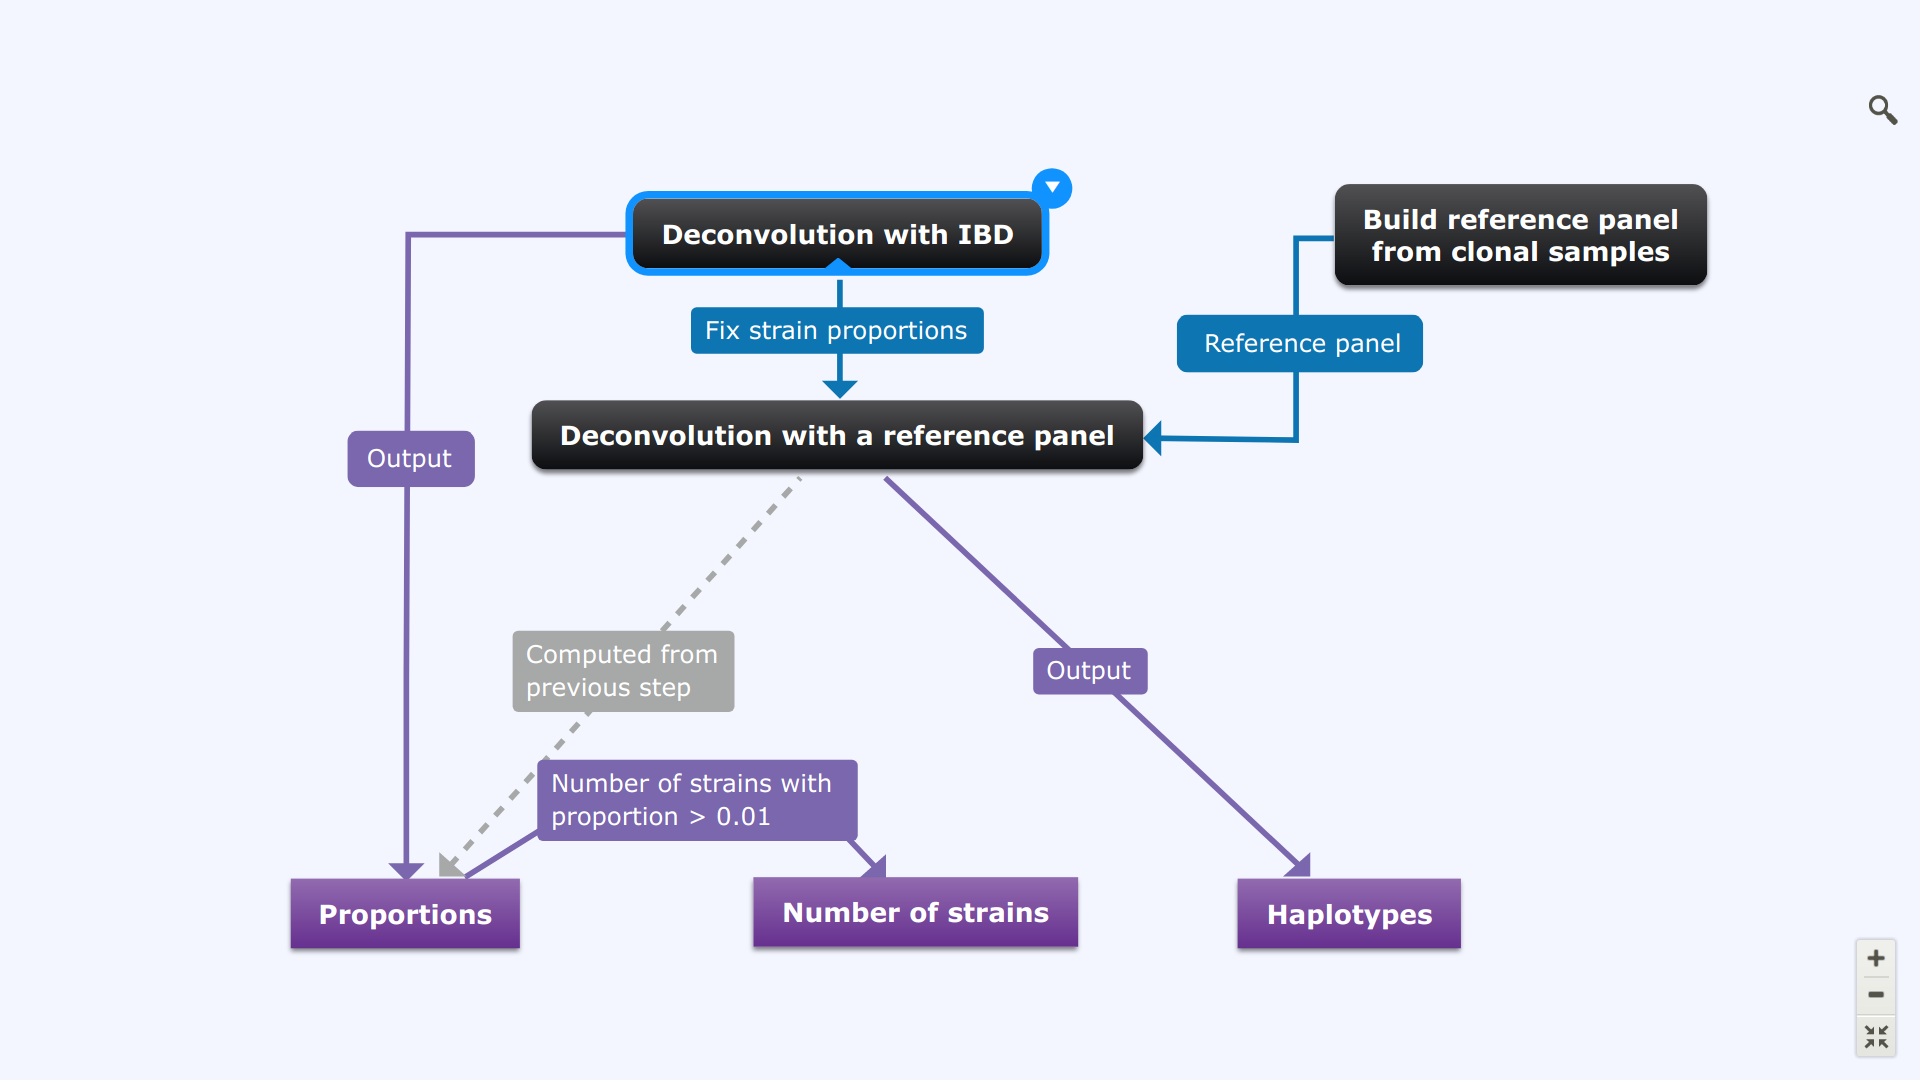
\includegraphics[width=0.7\textwidth]{scheme.png}}
   \caption{Deconvolution of field sample PD0577-C from Thailand.  (a) The profile of within-sample allele frequency along chromosomes 11 and 12 (black points) suggests a changing profile of IBD with three distinct strains, estimated to be at frequencies of $22\%$, $52\%$ and $26\%$ respectively (other chromosomes omitted for clarity); blue points indicate expected allele frequencies within the isolate.  However, the strains are inferred to be sibs of each other: green segments identify where all three strains are IBD; yellow, orange and dark orange segments identify the regions where one pair of strains are IBD but the others are not.  In no region are all three strains inferred to be distinct. (b) Summary of allele frequencies observed within the isolate shown as a scatter-plot of the numbers of reads supporting the reference (REF: x-axis) and alternative (ALT: y-axis) alleles.  A graphical description of the modules and workflows for \texttt{DEploidIBD} is given in Figure 1 - figure supplement 1.}\label{fig:fig1}
\end{figure}


\subsection{Validation}
Similar to \citep{Zhu2017}, we validated IBD-LD-DEploid using the same set of {\it in vitro} mixtures created by \citet{Wendler2015} to simulate mixed infections. This dataset includes 27 samples of which DNA extracted from four laboratory parasite lines: 3D7, Dd2, HB3 and 7G8, and mixed with different proportions (mixing proportions are available in supplementary material Fig~S1.1). To assess the performance, we experimented with different number of fitted strains (3 or 4). We repeated our experiment using the perfect reference panel for the lab mixtures, and found that apart from one experiment of 3 strains mixing with equal proportions, the rest of 26 experiment showed consistent results with the previous version. The new method struggled to converge to the correct solution for a specific set of mixing (see supplementary material), which were unlikely in the field.

To test the performance of IBD-LD-DEploid in a more realistic setting, we created {\it in silico} mixtures from 212 clonal samples of Asian origin with two proportions (25/75\% and 45/55\%) for 8071 sites from Chromosome 14. A further 20 randomly chosen samples were used for the reference panel. In order to compare the performance of the two methods at different level of relatedness between the two strains within the host, we set the first 25/50/75\% of the second haplotype the same as the first haplotype to mimic scenarios of low, moderate and high relatedness. To simulate data, we used empirical read depths and drew read counts for the two alleles from the binomial proportions.

% Expected effective k = 1.6 and 1.98.
To evaluate accuracy of estimates we used the effective number of strains, calculated as $1/\sum w_{i}^{2}$, which reflects the number and proportions of strains present. We found that for samples with strains of low or moderate relatedness. Both LD-only-DEploid and IBD-LD-DEploid correctly recover the effective number of strains. However, for samples with closely related strains, LD-only-DEploid tends to underestimate the effective number of strains when sequence coverages are low.

Our simulation show that IBD-LD-DEploid correctly recover the percentage of IBD regions of the mixed genomes (Figure~\ref{fig:benchmark}). As expected, IBD-LD-DEploid show similar diagnostics for switches and genotype errors: more switches and genotype errors in 45/55\% mixtures than 25/75\% mixtures. Moreover, we observe lower error rates in 45/55\% mixtures when the two strains are more related, which is expected because the deconvolution of distinct haplotypes length reduces. Therefore, we expect high genotype accuracy and low switch error rates, for field samples with unbalanced mixtures and closely related strains.


\begin{figure}[htp]
  \centering{}
  \subfloat[][]{
  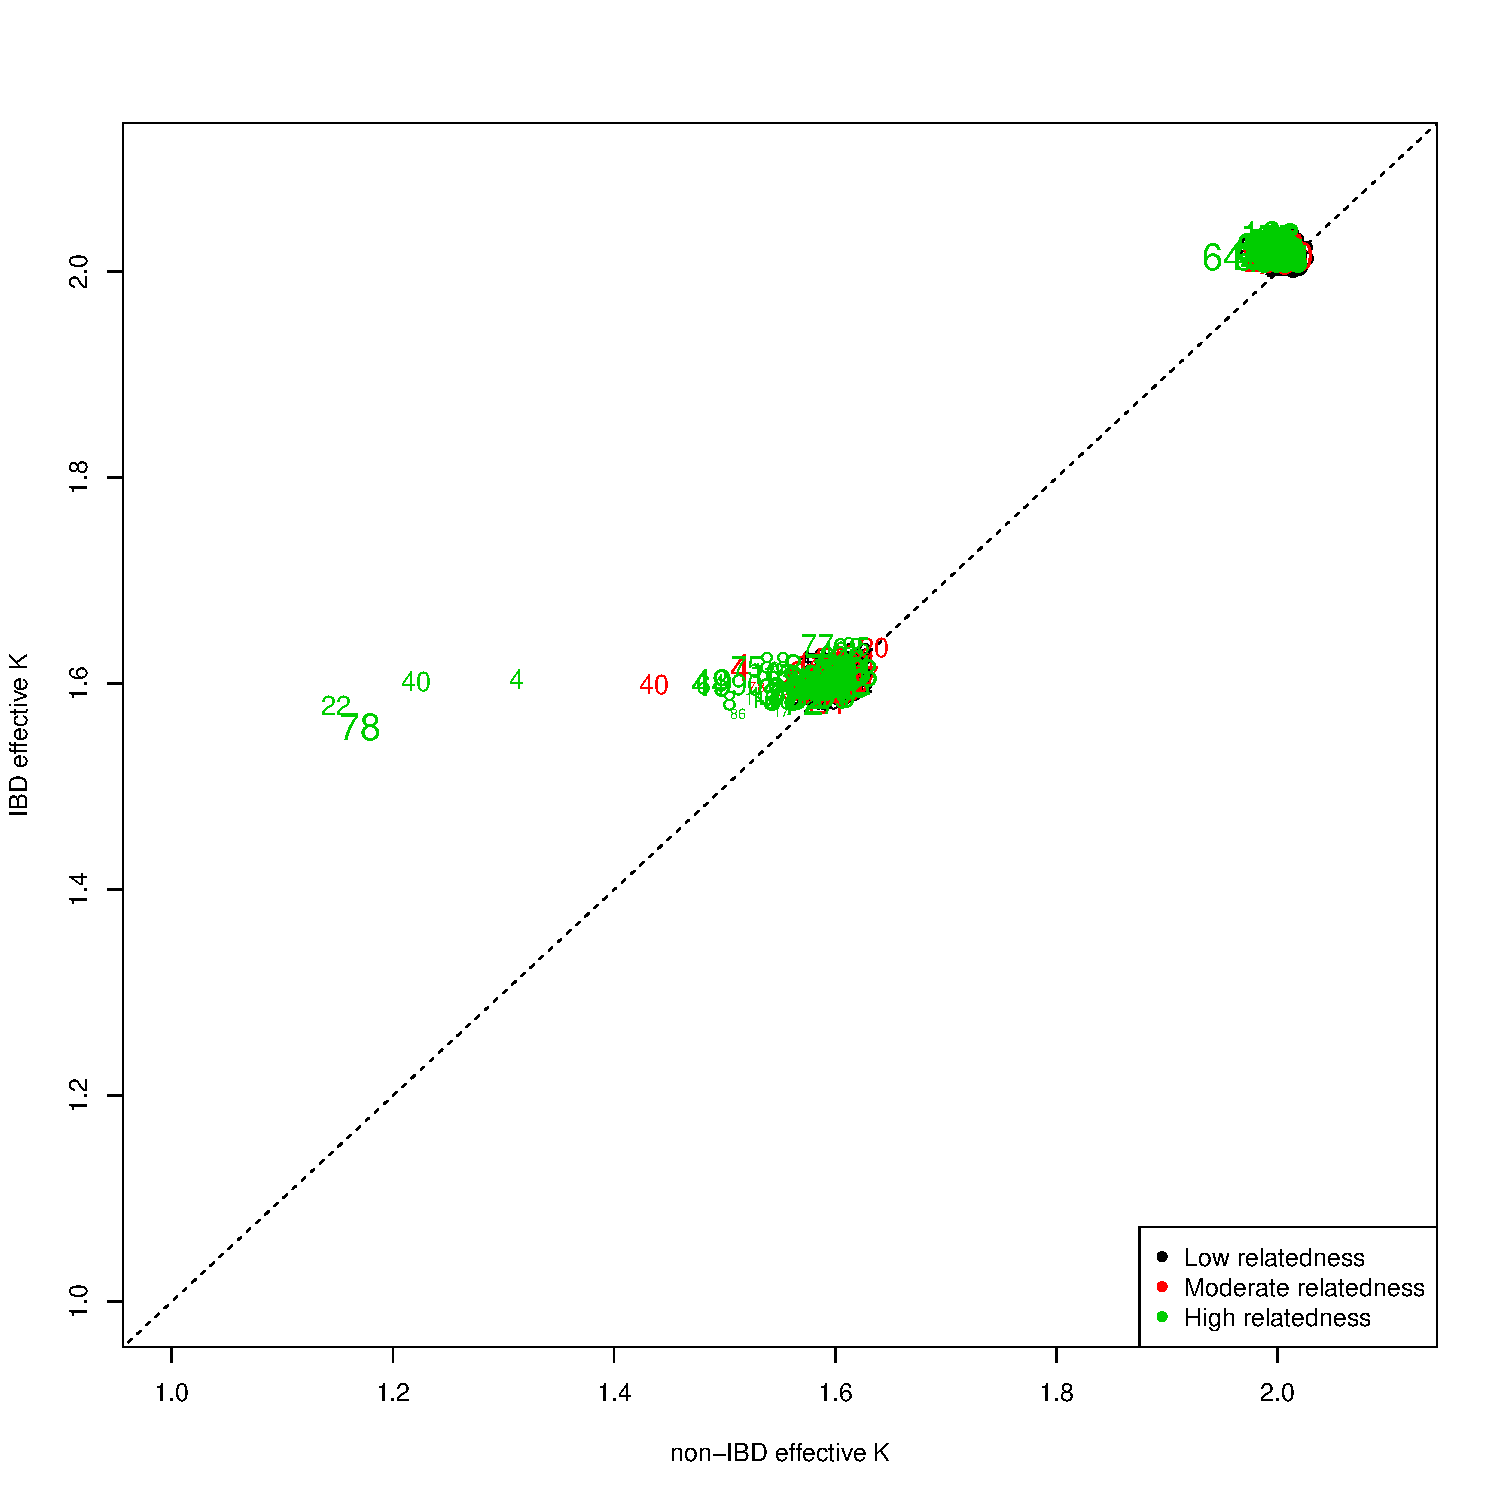
\includegraphics[width = 0.45\textwidth]{diagnositicPlot_of_effK_final.pdf}
  }
  \subfloat[][]{
  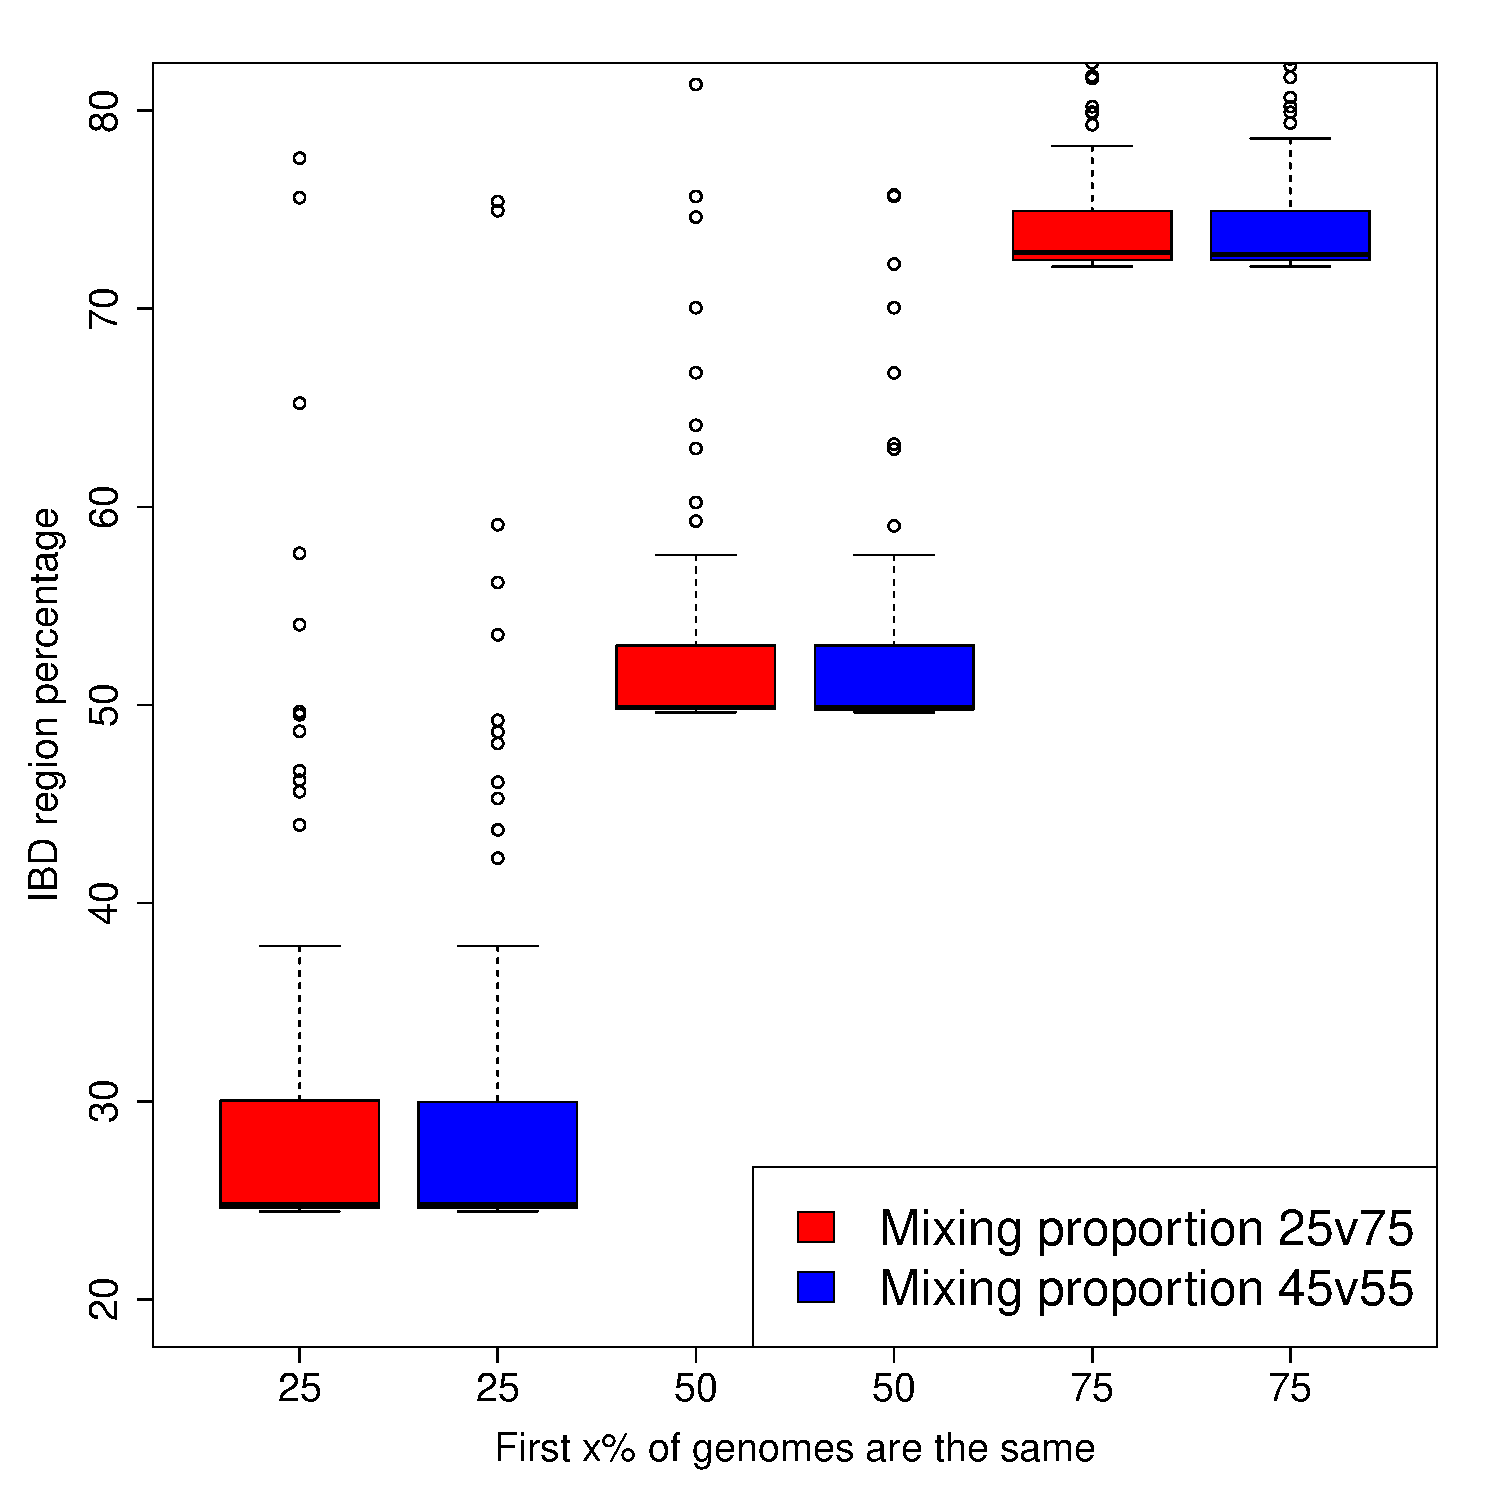
\includegraphics[width = 0.45\textwidth]{IBDprobs.pdf}
  }\\
  \subfloat[][]{
  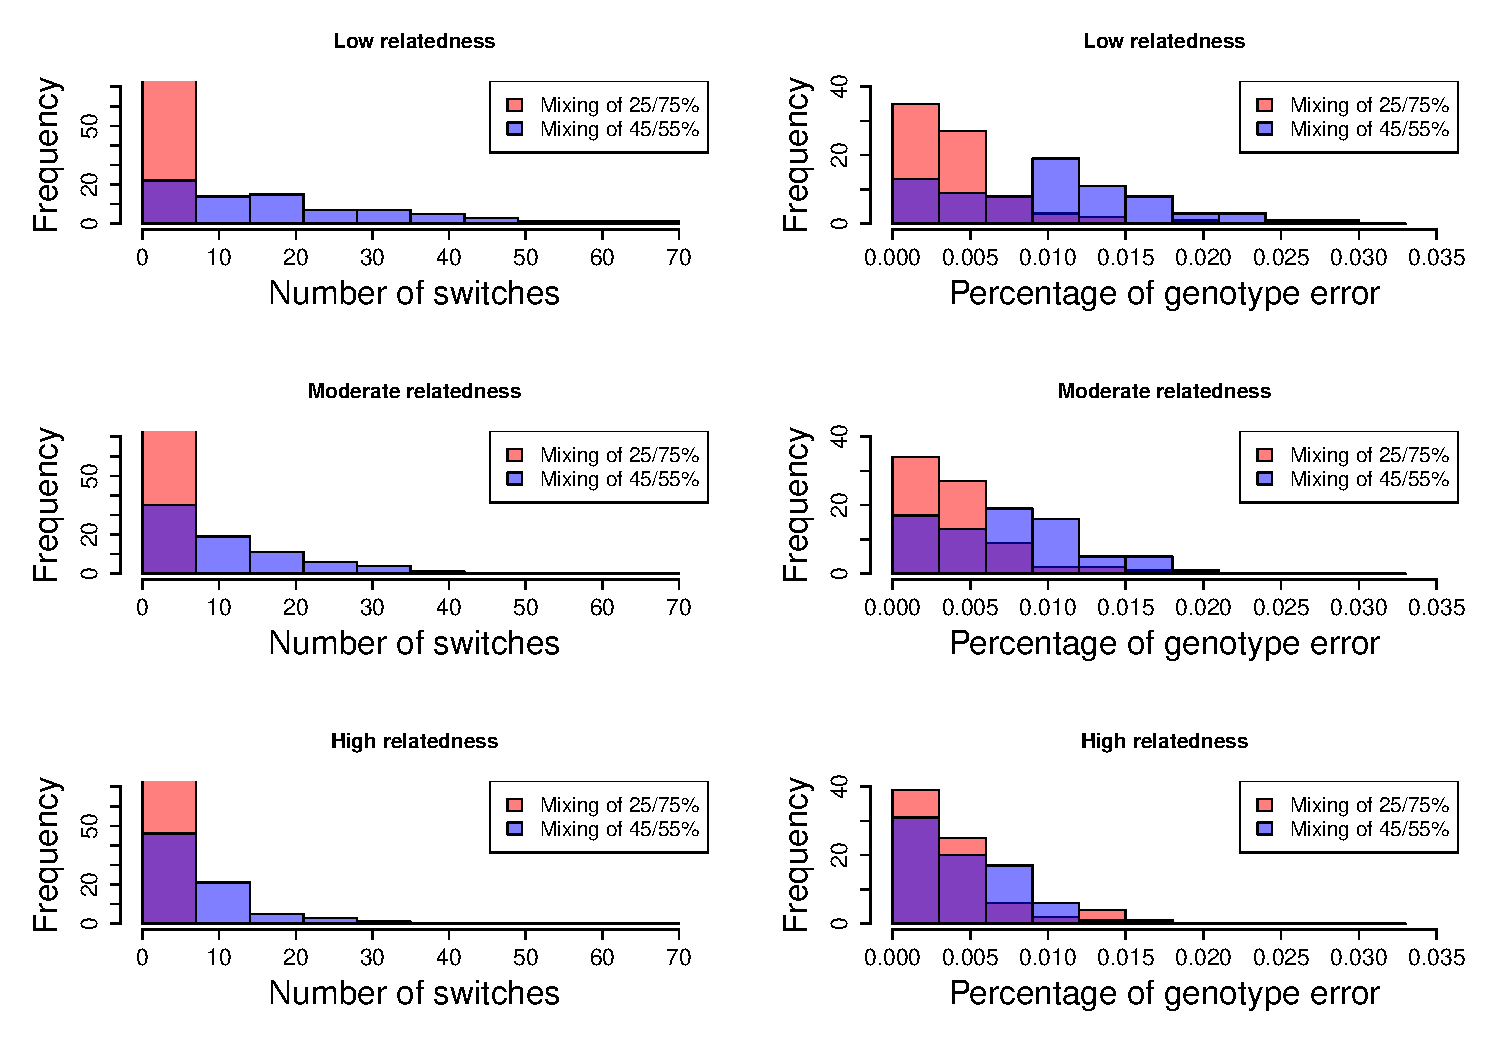
\includegraphics[width = 0.8\textwidth]{IBDHapError.pdf}
  }
  \caption{Simulation results. (a)Comparison of effective number of strains between LD-only-DEploid and IBD-LD-DEploid. (b)Expected and inferred percentage of IBD regions for IBD-LD-DEploid. (c) Histograms of switch error and genotype error across 76 simulated Pf3k samples for IBD-LD-DEploid. In all figures, we excluded eight cases out of the 100 experiments where simulated haplotypes were over 99\% identical and 16 cases where average coverage was below 20.
}\label{fig:benchmark}
\end{figure}




\section{Results}
\subsection{Application to {\it P. falciprium} data}

\donenarrative{1. Data source and preparation (i.e. cleaning).  Supplementary Figure 2 on importance of strong variant filtering.}

To estimate relative proportions and strain haplotypes we use IBD-LD-DEploid on high quality biallelic SNP data (both coding and non-coding variants tagged with PASS at the QUAL column in the VCF file) of the Pf3k \citep{Pf3k2016} and {\it P. vivax} Genome Variation dataset\citep{Pearson2016}, with 1,057,830 and 303,616 SNPs for {\it P. falciparum} and {\it P.vivax} respectively. We observe a small number of heterozygous sites with high coverage in the Pf3k data, which can potentially mislead our model to over-fit the data with additional strains. These poorly-genotyped variants are likely to be artefacts of mapping and genotype calling. We therefore identify potential outliers in all samples, and filter out common outliers in at least 50 samples -- 48,443 in total.

In order to improve the accuracy of the deconvolution process and improve efficiency, we first split the  data into groups, based on genetic similarity. We compute genetic distances between two samples following:
\begin{equation}
d(x, y) = \sum_{l}^{L}\textrm{WSAF}_{x,l} * (1-\textrm{WSAF}_{y,l}) + \textrm{WSAF}_{x,l} * (1-\textrm{WSAF}_{y,l})
\end{equation}
where $l$ represents an arbitrary locus, $L$ denotes the total number of loci, and $\textrm{WSAF}_{s,l}$ indicates the non-reference within-sample allele frequency for sample $s$ at locus $l$. $\textrm{WSAF}_{s,l}$ is then given by $\textrm{WSAF}_{s,l} = \frac{a_{s,l}}{r_{s,l}+a_{s,l}}$ where $a_{s,l}$ is the number of read counts supporting the alternative allele in sample $s$ at locus $l$, and $r_{s,l}$ is the number of read counts supporting the reference allele in sample $s$ at locus $l$.

We find that samples from the same geographical region differentiate into clear clusters. We use this initial grouping as the base for defining the reference panels that assist the deconvolution procedure. Our definition of geographical groups is
\begin{enumerate}
  \item Malawi, Congo.
  \item Ghana (Kassena).
  \item Nigeria, Senegal, Mali.
  \item The Gambia, Guinea, Ghana (Kintampo).
  \item Cambodia (Pursat), Cambodia (Pailin), Thailand (Sisakhet).
  \item Vietnam, Laos, Cambodia (Ratanakiri), Cambodia (Preah Vihear).
  \item Bangladesh, Myanmar, Thailand (Mae Sot), Thailand (Ranong).
\end{enumerate}

For the {\it P. vivax} data, we have the geographical groups as
\begin{enumerate}
  \item{} Thailand
  \item{} Indonesia, Malaysia, Papua New Guinea
  \item{} Cambodia, Vietnam, Laos
  \item the rest samples: Myanmar, China, Madagascar, Sri Lanka, Brazil and India.
\end{enumerate}



\narrative{2. Summary of findings within Pf and Pv. Figure 3: Rates of co-infection by geography and species.}
\textcolor{red}{TODO 2. Summary of findings within Pf and Pv. Figure 3: Rates of co-infection by geography and species.}



\narrative{3. Summary of findings about relatedness within mixed infections.  Figure 4.  Relatedness structure histogram showing peaks at 0.25, 0.5, etc. and relationship between mixed infection rate and sib-strain.}

\begin{figure}[htp]
  \centering{}
  \subfloat[][]{
    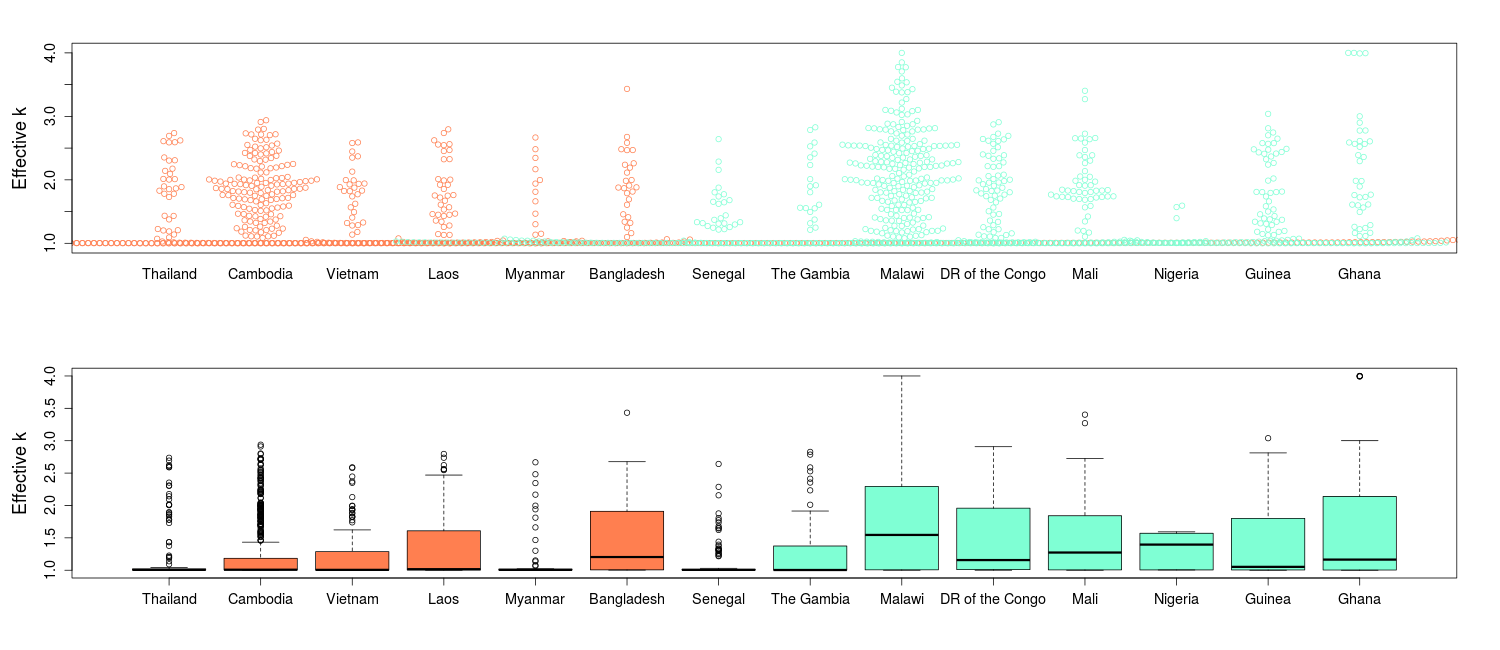
\includegraphics[width=0.7\textwidth]{beeswarm_effect_k.png}
  }\\
  \subfloat[][]{
  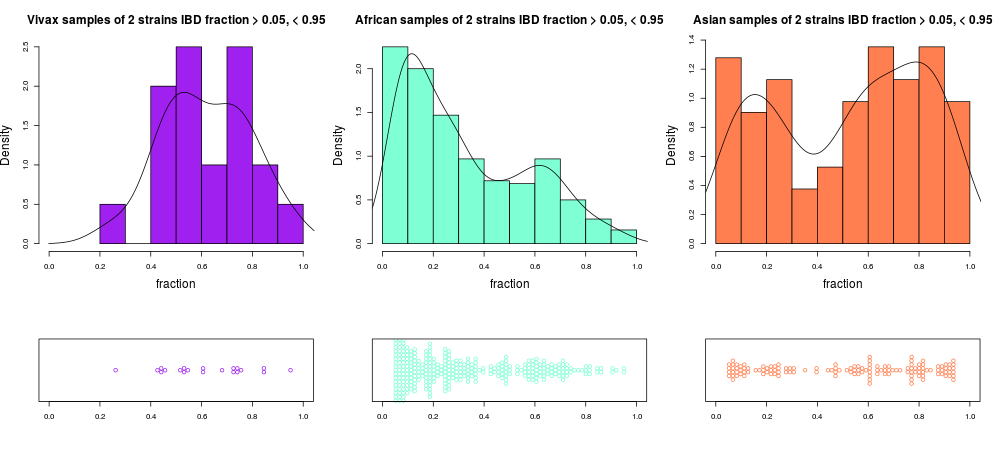
\includegraphics[width = 0.7\textwidth]{ibd_frac_hist.png}
  }\\
  \subfloat[][]{
    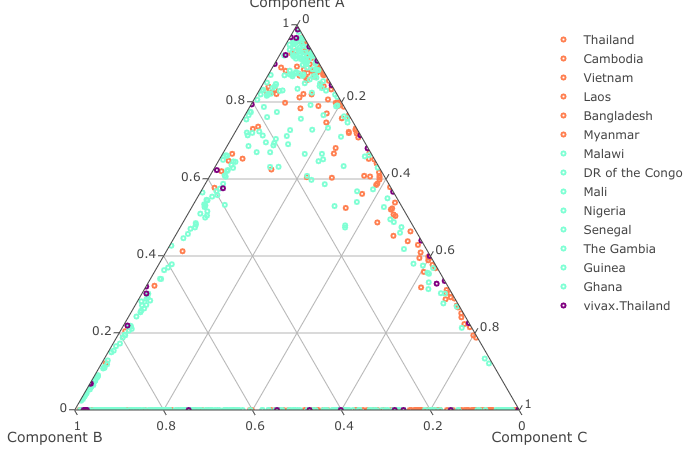
\includegraphics[width=0.7\textwidth]{ibdDistribution_withVivax.png}
  }\\
  %\subfloat[][]{
    %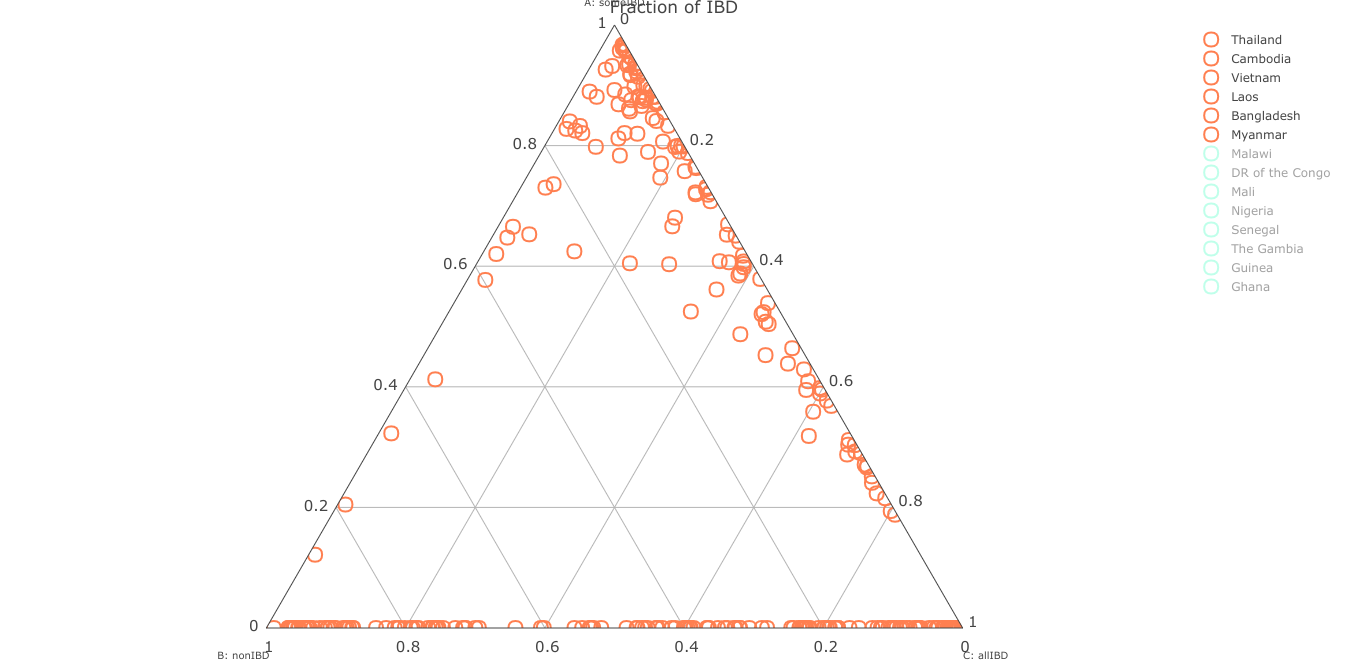
\includegraphics[width=0.8\textwidth]{ibdDistribution_asia.png}
  %}\\
  \caption{(a) Distribution of effective $k$ in each country. Countries in Asia show lower effective $k$ in Africa countries. Note Senegal and Gambia are similar to most Asia countries with low values of effective $k$. (b) Histograms of IBD fractions of two strain mixture samples. Relatedness structure of mixed samples peaks around 0.25, 0.5 suggest that mixed infections are caused by sib-strains. (c) Ternary plot of IBD fractions of all IBD, non-IBD and some-IBD of all mixed samples. Asia samples lean towards more IBD, Asia samples lean towards less IBD.}
  \label{fig:IBD_frac_hist}
\end{figure}







\subsection{Monitoring malaria epidemic from the IBD configuration probabilities}

\begin{figure}[htp]
  \centering{}
  \subfloat[][]{
  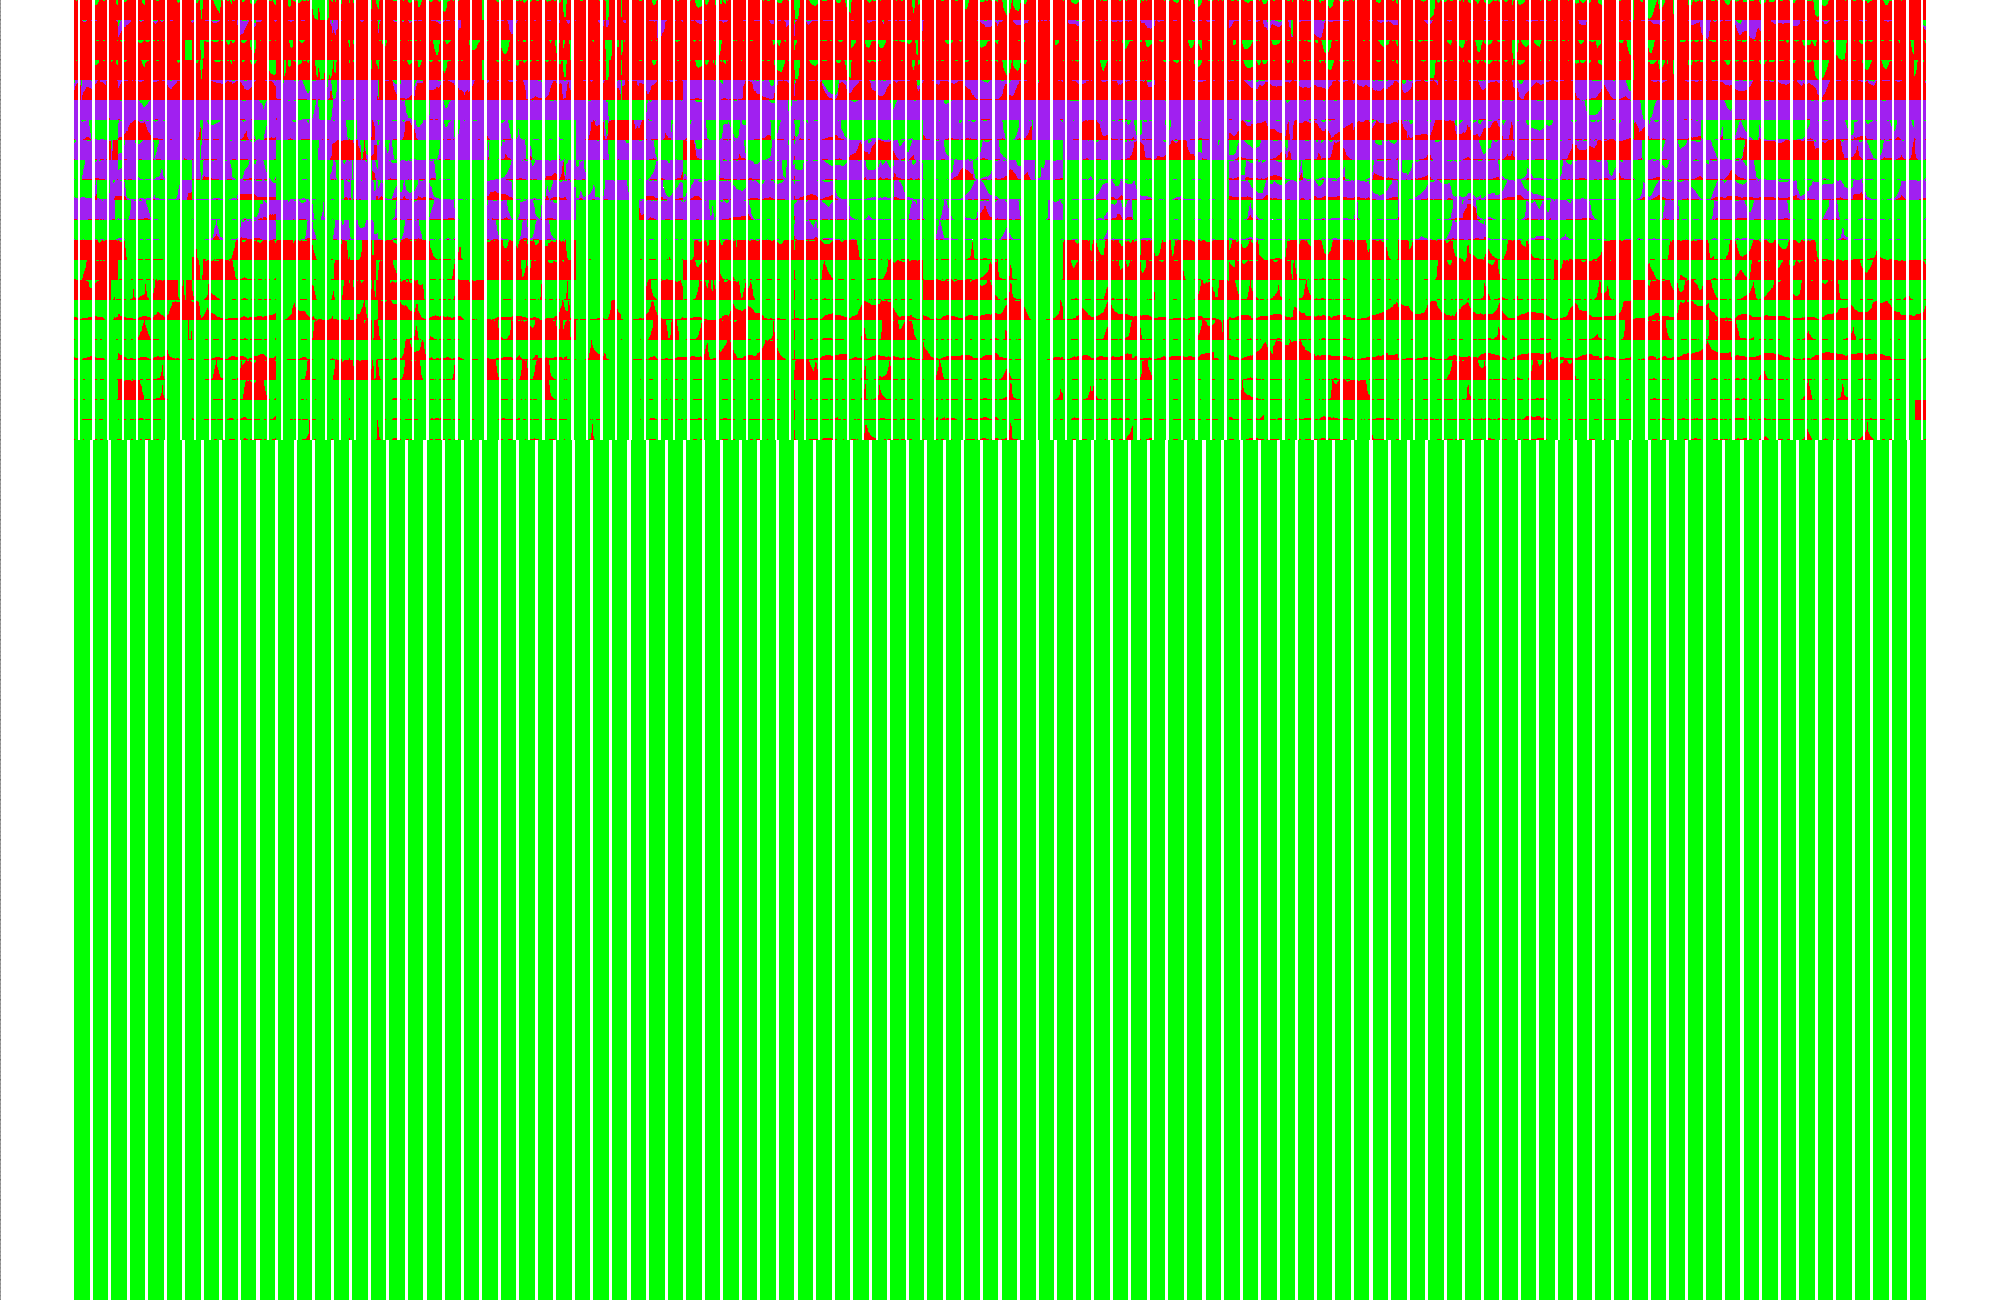
\includegraphics[width = 0.8\textwidth]{GambiaIBD.png}
  }\\
  \subfloat[][]{
  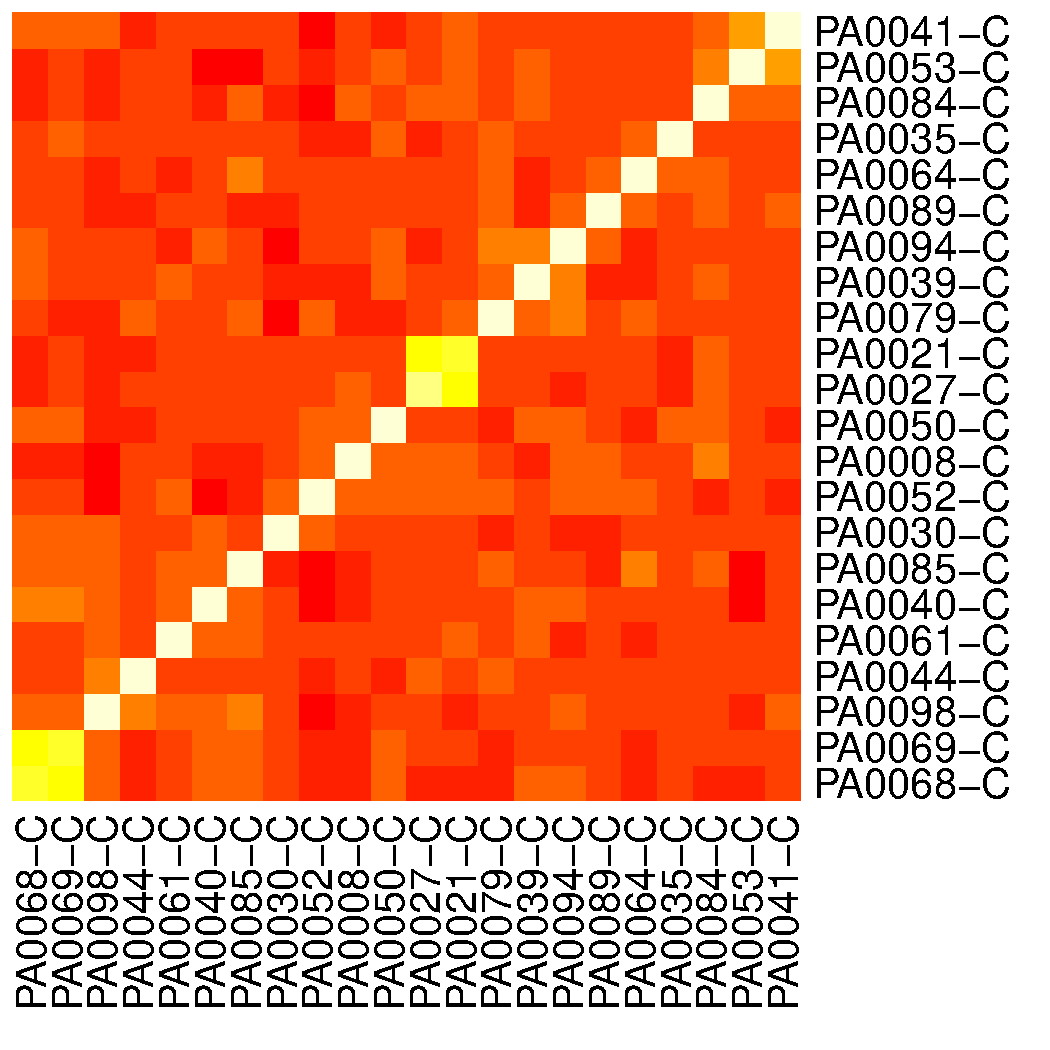
\includegraphics[width = 0.65\textwidth]{gambia_tmp.pdf}
  }\\
  \caption{(a) IBD fractions across genome of Gambia samples. Red purple and green colors indicate the fraction of the genomes are IBD. (b) Pairwise correlations of IBD fractions between mixed Gambia samples. The two yellow squares highlight two pairs of samples: PA0068-C and PA0069-C, PA0021-C and PA0027-C that share similar IBD configurations.}\label{fig:gambia}
\end{figure}

We show how the genomes of co-existing strains are related to each other, observing in some cases high levels of genetic relatedness or inbreeding. We see cases where heterozygosity is structured along the genome in a manner that suggests inbreeding, finding multiple cases of strains that are within 1-2 meioses of each other (Fig~\ref{fig:fig1}(a)). We envision that such a signature could be exploited in future micro-epidemiological studies to help in the inference of infection histories and transmission trees.

At the population level, we explore the malaria epidemic by stacking up all IBD posterior probabilities (Fig~\ref{fig:gambia}(a)). We observe striking variation in inbreeding patterns across populations with a mean inbreeding fraction range of \textcolor{red}{[0.07, 0.54]}. African countries, with the exception of The Gambia and Senegal, seem to have less inbred mixed infections, in agreement with the different levels of genetic diversity observed in each continent. These population-specific differences relate to the epidemiological setting of each region and provide a novel, and potentially important, source of information about local infection dynamics.

Between the mixed samples, we computed pairwise correlation between the IBD-fraction across genome. As expected, we observe high correlations in IBD profiles from 22 Malawi samples that had been sequenced twice through the MalariaGEN pipeline. We also observe similar high correlations between unique samples in Vietnam, Gambia, Cambodia and Bangladesh. We used threshold of 0.8 correlation to identify related infections. For example, in Figure~\ref{fig:gambia}(b), two pairs of sample, PA0068-C and PA0069-C, PA0021-C and PA0027-C show very strong correlations between the IBD-fraction across the genome. Samples PA0021-C and PA0027-C show very little evidence of inbreeding. On the other hand, we observe a strong negative correlation between the WSAF, which we speculate that both infections are caused by two mosquito carrying single strain of parasite, but the infection times are different; or one patent had been treated but the effect of drug appear differently, because the dominate strain in PA0021-C is the minor strain of PA0027-C, and vice versa. In the other case, parasite strains within samples PA0068-C and PA0069-C show strong evidence of IBD sharing, which can only happen when two people were bitten by the same mosquito, which is carrying two strains that have recombined within the mosquito. Interestingly, we observe the third strain in PA0068-C, which could mean that recombination is already happening again. Or we just don't observe it in PA0069-C.

%These samples are mixtures of two, with proportions of
%==> PA0021-C_newFilter_seed1_IBD.log <==
  %0.747591    3.23594e-09      0.252409    3.42703e-09

%==> PA0027-C_newFilter_seed1_IBD.log <==
  %0.860842    2.3895e-09      0.139158    2.52997e-09

%==> PA0068-C_newFilter_seed1_IBD.log <==
  %0.783381     0.0387533    4.0773e-05      0.177825

%==> PA0069-C_newFilter_seed1_IBD.log <==
  %0.665359    4.58131e-09      0.334641    4.92958e-09

%On average, two unrelated strains differ at 8000 places, and I found
%#> sum(PA0021.haps$h1 != PA0027.haps$h3)
%#[1] 380
%#> sum(PA0021.haps$h3 != PA0027.haps$h1)
%#[1] 119

%#> sum(PA0068.haps$h1 != PA0068.haps$h4)
%#[1] 820
%#> sum(PA0068.haps$h1 != PA0069.haps$h1)
%#[1] 368
%#> sum(PA0068.haps$h4 != PA0069.haps$h3)
%#[1] 438




\subsection{Malaria prevalence prediction}

We believe that the detailed characterization of mixed infections, in conjunction with localised epidemiological datasets like the ones provided by the Malaria Atlas Project [Bhatt et al., 2015], will improve our understanding of malaria epidemiology across the globe, permitting the identification of the major factors that modulate transmission in different countries. We also foresee that these methods will have important applications on the assessment of on-going interventions via genomic data [Volkman et al., 2012].

\textcolor{red}{update the linear model when cluster finishing }

Independence between effective k and IBD fraction (see Figure~.S*).

\narrative{4. Simulation results to analyse the relationship between prevalence, mixed infection rate and sib-strain rate.  Figure 5 summarising simulations.}


\begin{figure}[htp]
\centering
  \subfloat[][]{
  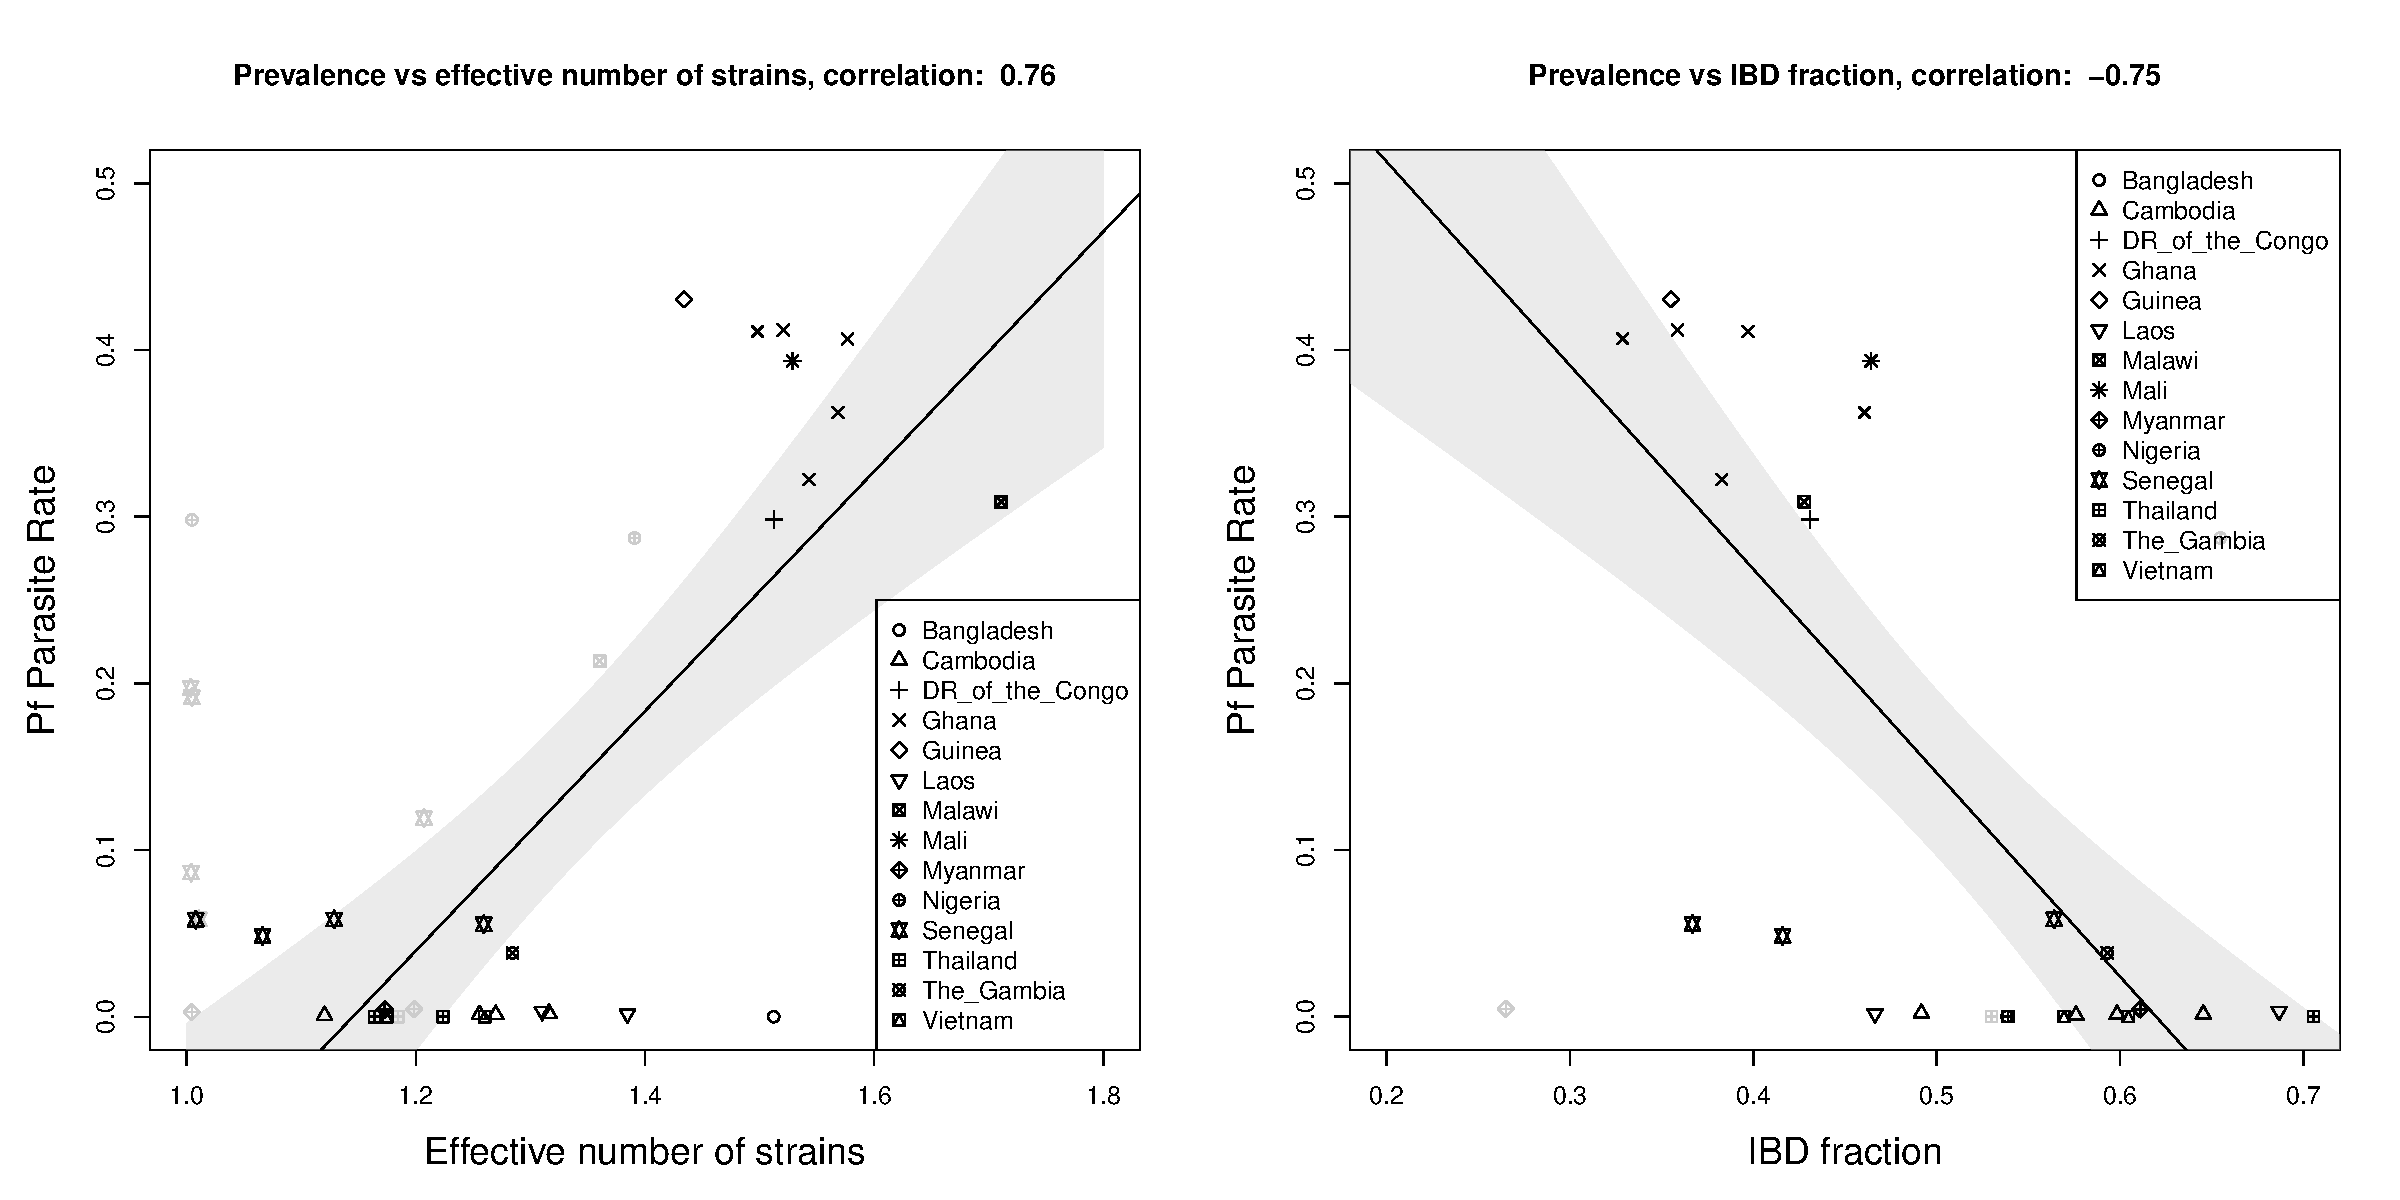
\includegraphics[width=0.8\textwidth]{prevelance.pdf}
}
%\\
  %\subfloat[][]{
  %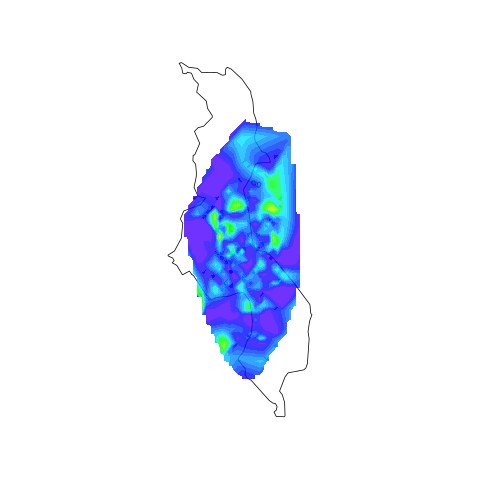
\includegraphics[width=0.8\textwidth]{Malawi.png}
%}
\caption{Black dots show African samples for modelling, red dots are the predicted values \textcolor{red}{1. update with vivax, 2. replace Malawi map with Africa map and Asia map}}
\end{figure}


\section{Discussion}
\textcolor{red}{To expand ...}
\narrative{1. Recap of main findings.}

\narrative{2. Relationship of mixed infection to prevalence v population size from simulations and interpretation of empirical data in the light of this.}

\narrative{3. Interpretation of within and between sample relatedness – does it reflect some feature of underlying biology?}

\narrative{4. Directions for integrating genomic data into efforts to map spatial and temporal changes in prevalence.}

The new method have greatly advanced current IBD methods for studying {\it Plasmodium} genomic dynamics within the host. It allows transitions between different pairwise IBD states, as well as to multiple strains IBD state. Moreover, DEploid returns inferred haplotypes, which enables researchers to investigate signals of selection in a high resolution.



\section{ACKNOWLEDGMENTS}
We thank the Pf3k consortium for valuable insights. The project is funded by the Wellcome Trust grant [100956/Z/13/Z] to GM.

\section{DISCLOSURE DECLARATION}
None declared.


\begin{thebibliography}{}

\bibitem[\protect\citeauthoryear{Bhatt}{Bhatt et~al.}{2015}]{Bhatt2015}
Bhatt, S. {\em et al}.
\newblock The effect of malaria control on Plasmodium falciparum in Africa between 2000 and 2015.
\newblock {\em Nature\/}~{\em 526}, 207--211, 2015.



\bibitem[\protect\citeauthoryear{Browning and Browning}{Browning and
  Browning}{2007}]{Browning2007}
Browning, S. R. and B.~L. Browning (2007)
\newblock Rapid and accurate haplotype phasing and missing-data inference for
  whole-genome association studies by use of localised haplotype clustering.
\newblock {\em Am. J. Hum. Genet.\/}~{\em 81\/}(5), 1084--1097.

\bibitem[\protect\citeauthoryear{Chang}{Chang et~al.}{2017}]{Chang2017}
\textcolor{black}{Change, H.~H. et al. (2017)
\newblock THE REAL McCOIL: A method for the concurrent estimation of the complexity of infection and SNP allele frequency for malaria parasites.
\newblock {\em PLoS Comput. Biol.\/}~{\em 13\/}(1), e1005348.}

\bibitem[\protect\citeauthoryear{Collins}{Collins}{2012}]{Collins2012}
Collins, W. E. (2012).
\newblock {\it Plasmodium knowlesi}: A malaria parasite of monkeys and humans.
\newblock {\em Annual Review of Entomology}~{\em 57\/}, 107--21.

\bibitem[\protect\citeauthoryear{Galinsky et~al.}{Galinsky et~al.}{2015}]{Galinsky2015}
Galinsky, K. {\em et al}. (2015)
\newblock COIL: a methodology for evaluating malarial complexity of infection using likelihood from single nucleotide polymorphism data.
\newblock {\em Malar. J.\/}~{\em14\/}(4), 1--9.

\bibitem[\protect\citeauthoryear{Hinch}{Hinch}{2011}]{Hinch2011}
Hinch, A. G. {\em et al}. (2011)
\newblock The landscape of recombination in African Americans.
\newblock {\em Nature\/}~{\em 476}, 170--175.

\bibitem[\protect\citeauthoryear{Henden}{Henden}{2016}]{Henden2016}
Henden, L. {\em et al}. (2016)
\newblock Detecting selection signals in {\it Plasmodium falciparum} using identity-by-descent analysis,
\newblock {\em bioRxiv.\/}, 088039.

\bibitem[\protect\citeauthoryear{Howes}{Howes}{2016}]{Howes2016}
Howes, R.E. {\em et al}. (2016)
\newblock Global Epidemiology of Plasmodium vivax
\newblock {\em Am. J. Trop. Med. Hyg\/}~{\em 95}, 15--34.

\bibitem[\protect\citeauthoryear{Jiang}{Jiang}{2011}]{Jiang2011}
Jiang, H. {\em et al}. (2011)
\newblock High recombination rates and hotspots in a {\it Plasmodium falciparum} genetic cross.
\newblock {\em Genome Biology.\/}~{\em 12}, R33.

\bibitem[\protect\citeauthoryear{Lopez}{Lopez}{2012}]{Lopez2012}
Lopez A. {\em et al}. (2012)
\newblock Genetic diversity of {\it Plasmodium vivax} and {\it Plasmodium falciparum} in Honduras.
\newblock {\em Malaria Journal.\/}~{\em 11}, 391.

\bibitem[\protect\citeauthoryear{Manske et~al.}{Manske et~al.}{2012}]{Manske2012}
Manske, M. {\em et al}. (2012)
\newblock Analysis of plasmodium falciparum diversity in natural infections by deep sequencing.
\newblock {\em Nature\/}~{\em 487\/}(7407), 375--379.

\bibitem[\protect\citeauthoryear{Miles et~al.}{Miles et~al.}{2016}]{Miles2016}
Miles, A. {\em et al}. (2015)
\newblock Indels, structural variation, and recombination drive genomic diversity in {\it Plasmodium falciparum}.
\newblock {\em Genome Res.\/}~{\em26\/}, 1288--1299.

\bibitem[\protect\citeauthoryear{Mu}{Mu}{2005}]{Mu2005}
Mu, J. {\em et al}. (2005)
\newblock Recombination Hotspots and Population Structure in {\it Plasmodium falciparum}.
\newblock {\em PLOS Biology.\/}~{\em 3}, e335.

\bibitem[\protect\citeauthoryear{Mueller et~al.}{Mueller et~al.}{2007}]{Mueller2007}
Mueller, I. {\em et al}. (2007)
\newblock {\it Plasmodium malariae} and {\it Plasmodium ovale} -- the ``bashful'' malaria parasites.
\newblock {\em Trends in Parasitology}~{\em 23\/} (6), 278--283.

\bibitem[\protect\citeauthoryear{Nair et~al.}{Nair et~al.}{2014}]{Nair2014}
Nair, S. {\em et al}. (2014)
\newblock Single-cell genomics for dissection of complex malaria infections
\newblock {\em Genome research.\/}~{\em 24}, 1028--1038.

\bibitem[\protect\citeauthoryear{Neafsey}{Neafsey}{2012}]{Neafsey2012}
Neafsey, D. {\em et al}.(2012)
\newblock The malaria parasite {\it Plasmodium vivax} exhibits greater genetic diversity than {\it Plasmodium falciparum}.
\newblock {\em Nature Genetics\/}~{\em 44\/}(9), 1046--1052.

\bibitem[\protect\citeauthoryear{O'Brien et~al.}{O'Brien et~al.}{2016}]{Jack2016}
O'Brien D. J. {\em et al}. (2016)
\newblock Inferring Strain Mixture within Clinical {\em Plasmodium falciparum} Isolates from Genomic Sequence Data.
\newblock {\em PLoS Comput. Biol.\/}~{\em 12\/}(6): e1004824.

\bibitem[\protect\citeauthoryear{O'Brien et~al.}{O'Brien et~al.}{2015}]{Jack2016Inbreeding}
O'Brien D. J. {\em et al}. (2016)
\newblock Approaches to estimating inbreeding coefficients in clinical isolates of {\it Plasmodium falciparum} from genomic sequence data.
\newblock {\em Malaria Journal\/}~{\em 15}:473.

\bibitem[\protect\citeauthoryear{Pearson et~al.}{Pearson et~al.}{2016}]{Pearson2016}
Pearson, R. D. {\em et al}. (2016)
\newblock {Genomic analysis of local variation and recent evolution in {\it Plasmodium vivax}}.
\newblock {\em Nat. Genet.\/}~{\em 48}, 959--964.

\bibitem[\protect\citeauthoryear{Rutledge}{Rutledge et~al.}{2017}]{Rutledge2017}
Rutledge. G. G., {\em et al}. (2017)
\newblock {\it Plasmodium} malariae and P. ovale genomes provide insights into malaria parasite evolution
\newblock {\em Nature.\/}~{\em 542}, 101--104.

\bibitem[\protect\citeauthoryear{Pf3k}{Pf3k}{2016}]{Pf3k2016}
The Pf3k Project: pilot data release 5 (2016)
\newblock {www.malariagen.net/data/pf3k-5} [accessed 1 June 2016]

\bibitem[\protect\citeauthoryear{Schaffner}{Schaffner}{2017}]{Schaffner2017}
Schaffner, S. F. {\em et al.} (2017)
\newblock {hmmIBD: software to infer pairwise identity by descent between haploid genotypes},
\newblock {\em bioRxiv}, doi:10.1101/188078.

\bibitem[\protect\citeauthoryear{Steenkeste}{Steenkeste}{2010}]{Steenkeste2010}
Steenkeste N. {\em et al.} 2010.
\newblock Sub-microscopic malaria cases and
mixed malaria infection in a remote area of high malaria endemicity in Rattanakiri Province, Cambodia: implication for
malaria elimination.
\newblock {\em Malar J}~{\em 9}: 108.


\bibitem[\protect\citeauthoryear{Wegmann}{Wegmann}{2011}]{Wegmann2011}
Wegmann, D. {\em et al}.(2011)
\newblock Recombination rates in admixed individuals identified by ancestry-based inference.
\newblock {\em Nature Genetics\/}~{\em 43\/}, 847--894.

\bibitem[\protect\citeauthoryear{Wendler}{Wendler}{2015}]{Wendler2015}
Wendler, J. (2015)
\newblock {\em Accessing complex genomic variation in} {P}lasmodium falciparum {\em natural infection}.
\newblock {Ph.\ D. thesis, University of Oxford.}

\bibitem[\protect\citeauthoryear{WHO}{WHO}{2016}]{WHO2016}
WHO. (2016)
\newblock {World Malaria Report 2015}.
\newblock {\em World Health Organization\/}.

\bibitem[\protect\citeauthoryear{Wong}{Wong}{2017}]{Wong2017}
Wong W., {\em et al}. (2017)
\newblock Genetic relatedness analysis reveals the cotransmission of genetically related {\it Plasmodium falciparum} parasites in Thiès, Senegal.
\newblock {\em Genome Medicine.\/}~{\em 9}:5. doi:10.1186/s13073-017-0398-0.

\bibitem[\protect\citeauthoryear{Zhu, Garcia, McVean}{Zhu et~al.}{2017}]{Zhu2017}
Zhu, J. S., {\em et al} (2017)
\newblock {Deconvoluting multiple infections in {\it Plasmodium falciparum} from high throughput sequencing data}.
\newblock {\em Bioinformatics\/}~{\em \/}btx530. doi: https://doi.org/10.1093/bioinformatics/btx530

\end{thebibliography}

\end{document}
